\section{Vision}

% \subsection{Initial Situation}
% In computer graphics, especially in games, an astonishingly large group of features are reccurring across all programs and genres.
% With the most obvious ones being water surfaces, cloudscapes and fire effects, they are present in almost any game. 
% Naturally, those features grew in complexity, customizability and computational demands over time.
% \\
% One of the core mechanics for achieving realistic results is called a \emph{\gls{volumetric} \gls{shader}}.
% A prototype such a \gls{shader} has been created in a previous project and will be used as base.

% \subsubsection{Previous Work}
% In a previous project, the process of creating a \gls{volumetric} \gls{shader} has already been researched and implemented in a prototype. Thanks to its high flexibility, different cloudscapes could be rendered by the same shader.

% \begin{figure}[ht]
%     \centering
%         \begin{minipage}{0.47\linewidth}
%             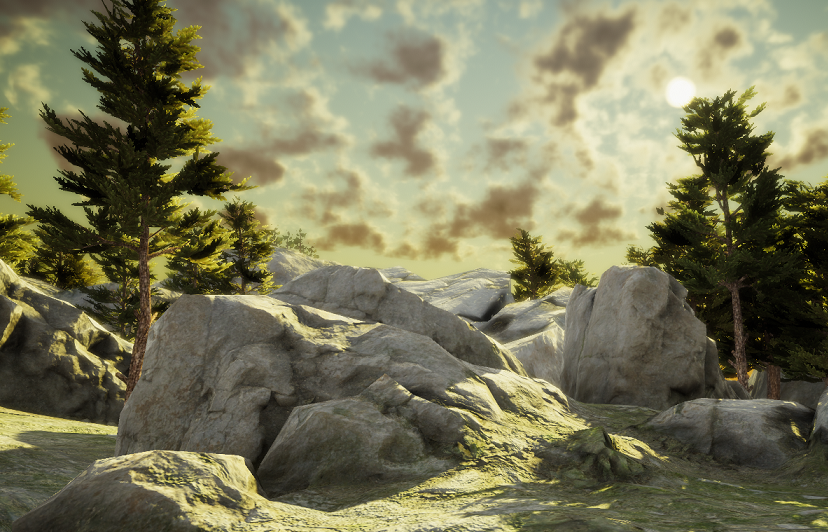
\includegraphics[width=\linewidth]{project2/project2-final.PNG}
%             \captionof{figure}{Result of the previous work's shader (Evening).}
%         \end{minipage}
%     \hfill
%         \begin{minipage}{0.47\linewidth}
%             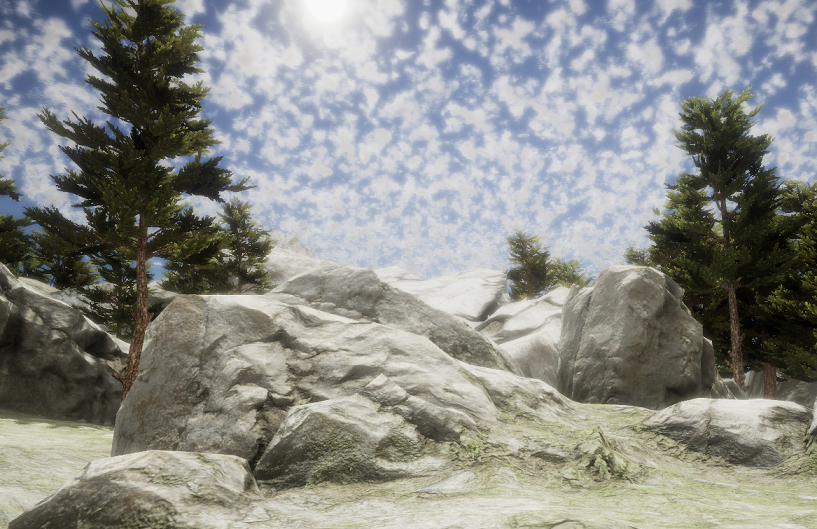
\includegraphics[width=\linewidth]{project2/project2-final2.PNG}
%             \captionof{figure}{Result of the previous work's shader (Day).}
%         \end{minipage}  
% \end{figure}

% \noindent
% During that project, some other important topics have been researched. Among those were \gls{volumetric} rendering, Perlin and Voronoi \gls{noisegeneration} algorithms, and a technique called \emph{\gls{raymarching}}.
% \\
% The implementations of those algorithms and methods will most likely be reused in this thesis and will be adapted and improved accordingly.

%  \subsection{Goals}
% \label{section:goals}
% As the title of the thesis suggests, this work will primarily focus on clouds and cloudscapes.
% The primary goal of the project is to research and implement rendering techniques for a real-time \gls{procedural} weather rendering system.
% \\
% The goals will be split into two distinct groups: mandatory and optional. However, this section only defines high-level goals. A detailed specification of all requirements can be found in \sectionref{section:requirements}.

% \subsubsection{Mandatory Goals}
% The following tasks must be accomplished during the project:
% \begin{itemize}
%     \item Understanding of different layers of clouds
%     \item Understanding of compute shaders
%     \item Implement a weather rendering system
%     \item Incorporate real-time weather data from \emph{meteoblue}
% \end{itemize}

% \subsubsection{Optional Goals}
% For further optional work, these tasks can be looked into:
% \begin{itemize}
%     \item Incorporate topological landscape models from \emph{swisstopo}
%     \item Automatic validation of realism of rendered cloudscapes
%     \item Automatic comparison of rendered cloudscapes and photographs
%     \item Automatic categorization of rendered cloudscapes
%     \item Performance optimization
% \end{itemize}

% \clearpage

% \subsection{Vision}
% This section defines a high-level vision for future work involving the results and implementations of this thesis. 
% As listed in the primary goals, the weather rendering system will be based on compute shaders.
% Compared to the prototype from the previous project, this is expected to result in a much better performance.
% That in turn, allows for a more complex and realistic model.
% \\
% With the incorporation of real-time weather data and the use of topological landscape data, any given weather scenario could be simulated and rendered.
% The desired outcome ideally looks similar to the image depicted in \autoref{img:rendered1}.
% A rendered version of such a cloud system can look elusively realistic compared to an actual photograph, like in \autoref{img:photo1}.
% \begin{figure}[ht]
%     \centering
%         \begin{minipage}{0.47\linewidth}
%             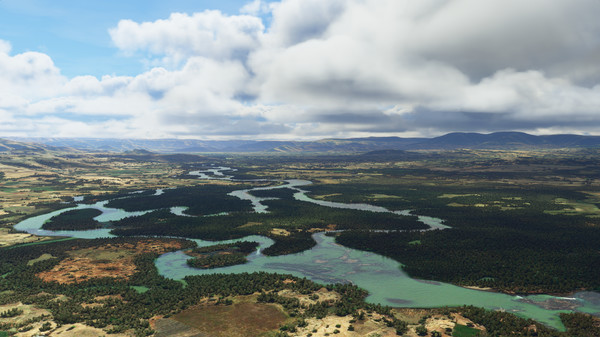
\includegraphics[width=\linewidth]{msfs-ref1.jpg}
%             \captionof{figure}{A rendered image of volumetric clouds \protect\cite{img:rendered:clouds01}.}
%             \label{img:rendered1}
%         \end{minipage}
%     \hfill
%         \begin{minipage}{0.47\linewidth}
%             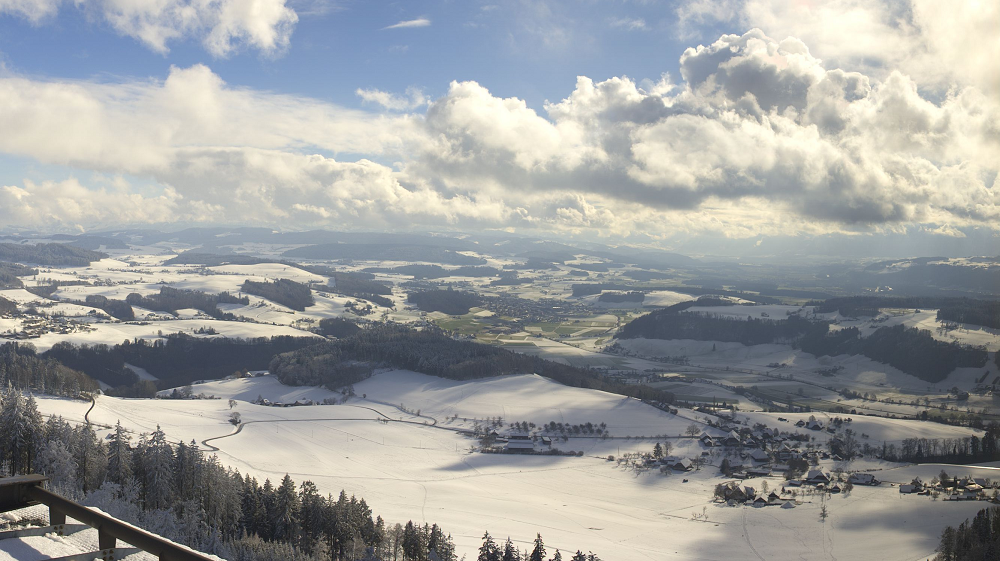
\includegraphics[width=\linewidth]{roundshot2021-01-18-12-50-cropped.png}
%             \captionof{figure}{A photographic reference of clouds \protect\cite{img:photo:clouds01}.}
%             \label{img:photo1}        
%         \end{minipage}  
% \end{figure}
% \\
% The first thought about the practical use of a fully-fledged volumetric cloud system might be a video game, since clouds are often a significant part of outdoor scenery in games.
% However, for this thesis it is intended that the knowledge and results acquired during the given period will be used to recreate a lifelike weather system instead.
% \\
% To accurately reflect a weather system, conditions like precipitation, wind and cloudiness will be considered. This data is obtained from the firm \emph{meteoblue}.

% \subsection{Educational Objectives}
% Educational objectives include \gls{shader} programming, knowledge about \gls{computeshader}s, rendering techniques, common algorithms used in computer graphics like \gls{noisegeneration}, a general understanding of aspects needed to create a complete weather system and finally the incorporation of real-time data from a third party.

% \subsection{Used Software and Tools}
% All documentation will be written in \gls{latex} with Visual Studio Code.
% The \gls{shader} will be implemented in Unity. The chosen \gls{shader} language is \gls{hlsl}.
% For the presentation, Microsoft PowerPoint will be used.